%%%%%%%%%%%%%%%%%%%%%%%%%%%%%%%%%%%%%%%%%%
%%%                                    %%%
%%% ©ablona bakal\'{a}\v{r}sk\'{e} pr\'{a}ce na MFF UK %%%
%%%                                    %%%
%%% (c) Frantiąek ©trupl, 2005         %%%
%%%                                    %%%
%%%%%%%%%%%%%%%%%%%%%%%%%%%%%%%%%%%%%%%%%%

%%% POZOR: Úprava bakal\'{a}\v{r}sk\'{e} pr\'{a}ce je z\'{a}visl\'{a} rovn\v{e}ľ na volb\v{e} jednostrann\'{e}ho resp. oboustrann\'{e}ho tisku.
%%%        Bliľąi informace naleznete v dokumentu Úprava bakal\'{a}\v{r}sk\'{e} pr\'{a}ce, kter\'{y} se nal\'{e}z\'{a} na adrese:
%%%        http://www.mff.cuni.cz/studium/obecne/bplayout/pok12mo4.pdf

\documentclass[12pt,a4paper,twoside,notitlepage]{article}
%\pagestyle{headings}
\pagestyle{plain}

\oddsidemargin 1.5cm
\evensidemargin 0.8cm


%%%\frenchspacing % aktivuje pouľit\'{i} n\v{e}kter\'{y}ch \v{c}esk\'{y}ch typografick\'{y}ch pravidel

%%%\usepackage[latin2]{inputenc} % nastavuje pouľit\'{e} kódov\'{a}n\'{i}, uľivatel\'{e} Windows zam\v{e}n\'{i} latin2 za cp1250
%%%\usepackage{czech}
%\usepackage{a4wide} % nastavuje standardn\'{i} evropsk\'{y} form\'{a}t str\'{a}nek A4

%\usepackage[inner=4cm]{geometry} % nastaven\'{i} dan\'{e} velikosti okraj\r{u}

%\addtolength{\hoffset}{3cm}

%\oddsidemargin 1.5cm
%\evensidemargin 0.8cm


\usepackage{index}     % indexing
\newindex{not}{notx}{notd}{Index of symbols}

\usepackage[T1]{fontenc}
\usepackage{nameref}
\usepackage[square]{natbib}
\usepackage{url}
\usepackage{nomencl}
\usepackage{multicol}
\usepackage{array}
\usepackage{colortbl}
\usepackage{amsthm}
\usepackage{verbatim}
\usepackage{wrapfig}
\usepackage{tocloft}



\usepackage{minted}

\usepackage{bigfoot}
\usepackage{hyperref}

\usepackage[xetex]{graphicx}

\usepackage{rotating}
\usepackage{longtable}
\usepackage{multirow}
\usepackage{threeparttable}

\usepackage[log-declarations=false]{xparse}
\usepackage[quiet]{fontspec}
\usepackage{xltxtra}
\setsansfont{Calibri}
\setmonofont{Consolas}

\def\myauthor{Jan Dědek}
\def\mytitle{Semantic Annotations}
\def\mysupervisor{Prof. RNDr. Peter Vojtáš, DrSc.}
\def\mydepartment{Department of Software Engineering}

\hypersetup{pdftitle=\mytitle}
\hypersetup{pdfauthor=\myauthor}



%footurl
\newcommand{\footurl}[1]{\footnote{\url{#1}}}


%sectiondoubleref
\newcommand{\sectiondoubleref}[1]{\nameref{#1} (Section~\ref{#1})} 


%openright
\let\openright=\cleardoublepage


%definition
\theoremstyle{definition}
\newtheorem{definition}{Definition}
\newtheorem{theorem}{Theorem}



% Tato makra přesvědčují mírně ošklivým trikem LaTeX, aby hlavičky kapitol
% sázel příčetněji a nevynechával nad nimi spoustu místa. Směle ignorujte.
\makeatletter
\def\@makechapterhead#1{
  {\parindent \z@ \raggedright \normalfont
   \Huge\bfseries \thechapter. #1
   \par\nobreak
   \vskip 20\p@
}}
\def\@makeschapterhead#1{
  {\parindent \z@ \raggedright \normalfont
   \Huge\bfseries #1
   \par\nobreak
   \vskip 20\p@
}}
\makeatother


% Toto makro definuje kapitolu, která není očíslovaná, ale je uvedena v obsahu.
\def\chapwithtoc#1{
\chapter*{#1}
\addcontentsline{toc}{chapter}{#1}
}



%\usepackage{graphicx, newalg, subfigure}
%\usepackage{wasysym}
%\usepackage{amssymb}
%\usepackage{multirow}
%\usepackage{verbatim}
%\usepackage{color}
%\usepackage{fancyvrb}
%\usepackage{listings}
%\usepackage{url}
%

\newcommand{\TheTitle}{Semantic Annotations}
%\newcommand{\TheTitleBrokenA}{Methods for effective querying of RDF data}
%\newcommand{\TheTitleBrokenB}{Methods for effective querying of RDF data}

\newcommand{\TheAuthor}{Mgr. Jan D\v{e}dek}
\newcommand{\TheSupervisor}{Prof. RNDr. Peter Vojt\'{a}\v{s}, DrSc.}
\newcommand{\TheAuthorMail}{dedek@ksi.mff.cuni.cz}
\newcommand{\TheSupervisorMail}{dedek@ksi.mff.cuni.cz} 

\newcommand{\uri}[1]{{\texttt{#1}}}
\newcommand{\triple}[3]{$<$\uri{#1},\uri{#2},\uri{#3}$>$}
\newcommand\ns[1]{\texttt{#1}}
\newcommand{\xbegincenter}[0]{\begin{center}}
\newcommand{\xendcenter}[0]{\end{center}}


\def \TODO#1{\textbf{\textcolor{red}{ TODO - #1}}}
\def \X{\mathcal{X}}
\def \S{\mathcal{S}}
\def \U{\mathcal{U}}
\def \r{\widehat{r}}
\def \smallHeading#1{\textbf{#1}\par}




%\newindex{default}{idx}{ind}{Rejst\v{r}\'{i}k} % zav\'{a}d\'{i} rejst\v{r}\'{i}k v p\v{r}\'{i}pad\v{e} pouľit\'{i} bal\'{i}ku index

\title{\TheAuthor}   % tyto dv\v{e} poloľky jsou zde v podstat\v{e} form\'{a}ln\v{e}, ve skute\v{c}nosti nejsou nikde 
\author{\TheTitle} % d\'{a}le v dokumentu pouľity

%\date{}

\begin{document}




%%%%%%%%%%%%%%%%%%%%%%%%%%%%%%%%%%%%%%%%%%%%%%%%%%%%%%%%%
%%%  TITLE PAGE
%%%%%%%%%%%%%%%%%%%%%%%%%%%%%%%%%%%%%%%%%%%%%%%%%%%%%%%%%

\begin{titlepage}
\begin{center}
\ \\

\vspace{15mm}

\large
Charles University in Prague\\
Faculty of Mathematics and Physics\\

\vspace{5mm}

{\Large\bf Abstract of Doctoral Thesis}

\vspace{10mm}

%%% Aby vloľn\'{i} loga vąe spr\'{a}vn\v{e} fungovalo, je t\v{r}eba m\'{i}t soubor logo.eps nahran\'{y} v pracovn\'{i}m adres\'{a}\v{r}i,
%%% tj. v adres\'{a}\v{r}i, kde se nach\'{a}z\'{i} p\v{r}ekl\'{a}dan\'{y} zdrojov\'{y} soubor. Soubor logo.eps je moľn\'{e} z\'{i}skat nap\v{r}.
%%% na adrese: http://www.mff.cuni.cz/fakulta/symboly/logo.eps

\includegraphics[scale=0.3]{../finall/style/logo} 

\vspace{15mm}

%\normalsize
{\Large \TheAuthor}\\ % doplňte vaąe jm\'{e}no
\vspace{5mm}
{\Large\bf \TheTitle} \\
%\bigskip
\vspace{5mm}
Department of Software Engineering\\ % doplňte n\'{a}zev katedry \v{c}i \'{u}stavu
%%%\end{center}
\vspace{15mm}

%%%\begin{center}
{
\large
\noindent Supervisor: \TheSupervisor 
}
%%%\end{center}
\vspace{1mm} 

\vspace{20mm}

%%%\begin{center}
2012 % doplňte rok vzniku vaą\'{i} bakal\'{a}\v{r}sk\'{e} pr\'{a}ce
\end{center}

\end{titlepage} % zde kon\v{c}\'{i} \'{u}vodn\'{i} strana

%%%%%%%%%%%%%%%%%%%%%%%%%%%%%%%%%%%%%%%%%%%%%%%%%%%%%%%%%
% INFO PAGE
%%%%%%%%%%%%%%%%%%%%%%%%%%%%%%%%%%%%%%%%%%%%%%%%%%%%%%%%%

\normalsize % nastaven\'{i} norm\'{a}ln\'{i} velikosti fontu
%\pagenumbering{none} 
\pagestyle{empty}
\setcounter{page}{2} % nastaven\'{i} \v{c}\'{i}slov\'{a}n\'{i} str\'{a}nek

\cleardoublepage

\noindent Doktorsk\'{a} pr\'{a}ce byla vypracov\'{a}na v r\'{a}mci doktorsk\'{e}ho studia, kter\'{e} ucha\-ze\v{c} absolvoval na Kated\v{r}e softwarov\'{e}ho in\v{z}en\'{y}rstv\'{i} Matematicko-fyzik\'{a}ln\'{i} fakulty Univerzity Karlovy v Praze v letech 2007--2012.

\vspace{5mm}

\noindent
\begin{tabular}{ll}
{ Uchaze\v{c}:}&\TheAuthor \\
&Katedra softwarov\'{e}ho in\v{z}en\'{y}rstv\'{i}\\
&MFF UK\\
&Malostransk\'{e} n\'{a}m. 25, 118 00 Praha 1 \\
%&bednarek@ksi.mff.cuni.cz \\
%\hspace*{10mm}Matematicko-fyzik\'{a}ln\'{i} fakulta\\
%\hspace*{10mm}Univerzita Karlova v Praze \\
& \\
{ Obor studia:}&I-2 -- Softwarov\'{e} syst\'{e}my \\
& \\
{ P\v{r}edseda oborov\'{e} rady:}&Prof. Ing. Franti\v{s}ek Pl\'{a}\v{s}il, DrSc. \\
&Katedra softwarov\'{e}ho in\v{z}en\'{y}rstv\'{i}\\
&MFF UK\\
&Malostransk\'{e} n\'{a}m. 25, 118 00 Praha 1 \\
& \\
{ \v{S}kolitel:}&\TheSupervisor \\
&Katedra softwarov\'{e}ho in\v{z}en\'{y}rstv\'{i}\\
&MFF UK\\
&Malostransk\'{e} n\'{a}m. 25, 118 00 Praha 1 \\
%&kral@ksi.mff.cuni.cz \\
&\\
{ Oponenti:}
&Dr. Diana Maynard\\
&Department of Computer Science\\
&University of Sheffield, United Kingdom\\
&Regent Court, 211 Portobello, Sheffield S1 4DP\\
&e-mail: diana@dcs.shef.ac.uk\\


\\&Doc. Ing. Filip \v{Z}elezn\'{y}, Ph.D.
\\&Katedra Kybernetiky, Fakulta elektrotechnick\'{a}
\\&\v{C}esk\'{e} vysok\'{e} u\v{c}en\'{i} technick\'{e} v Praze
\\&Karlovo n\'{a}m\v{e}st\'{i} 13
\\&121 35 Praha 2
\\&e-mail: zelezny@fel.cvut.cz


%&prof. Ing. Petr Berka, CSc. \\
%&Katedra informa\v{c}n\'{i}ho a znalostn\'{i}ho in\v{z}en\'{y}rstv\'{i} \\ 
%&Vysok\'{a} \v{s}kola ekonomick\'{a} v Praze \\
%&n\'{a}m. W.Churchilla 4, 130 67 Praha 3\\
%&berka@vse.cz  \\
%
%\\&prof. Yasushi Kiyoki
%\\&Department of Environmental Information 
%\\& Keio University,
%\\& 5322 Endo, Fujisawa-shi, Kanagawa, 252-0816  Japan 
%\\&kiyoki@mdbl.sfc.keio.ac.jp 
\end{tabular}

\vspace{4mm}

\noindent Autorefer\'{a}t byl rozesl\'{a}n dne

\noindent Obhajoba se kon\'{a} dne~\quad~\quad~\quad~\quad~\quad~v~\quad~\quad~\quad~hodin p\v{r}ed komis\'{i} pro obhajoby diserta\v{c}n\'{i}ch prac\'{i} v oboru I-2 -- Softwarov\'{e} syst\'{e}my na Matematicko-fyzik\'{a}ln\'{i} fakult\v{e} Univerzity Karlovy, Malostransk\'{e} n\'{a}m. 25, Praha 1, v m\'{i}stnosti \v{c}.~\quad~\quad~.

\noindent S disertac\'{i} je mo\v{z}n\'{e} se sezn\'{a}mit na studijn\'{i}m odd\v{e}len\'{i} MFF UK, Ke Karlovu~3, Praha 2.

%%%%%%%%%%%%%%%%%%%%%%%%%%%%%%%%%%%%%%%%%%%%%%%%%%%%%%%%%%%%%%%%%%%%%%%
% Body text
%%%%%%%%%%%%%%%%%%%%%%%%%%%%%%%%%%%%%%%%%%%%%%%%%%%%%%%%%%%%%%%%%%%%%%%

\cleardoublepage

\pagestyle{plain}
\pagenumbering{arabic}
\setcounter{page}{5}


\section{Introduction}

\graphicspath{{../img/ch10/}}


Four relatively separate topics are presented in the thesis and the discipline of Information Extraction is the central point of them. Each topic represents one particular aspect of the Information Extraction discipline.

The first two topics are focused on our information extraction methods based on deep language parsing. The first topic relates to how deep language parsing was used in our first method in combination with manually designed extraction rules.

The second topic deals with an alternative extraction method based on machine learning. An inductive procedure was developed based on Inductive Logic Programming (ILP), which allows automated learning of extraction rules from a learning collection.

The idea of the Semantic Web was the strongest motivation of our research from the very beginning. We wanted to exploit information extraction techniques to speed up the semantic web evolution. The third topic of the thesis presents even more than that. The core of the extraction method was experimentally reimplemented using semantic web technologies. Therefore not only the result of information extraction but also the extraction procedure itself is realized using semantic web technologies. The main advantage of this approach is the possibility to save the extraction rules in so called shareable extraction ontologies.

The last topic of the thesis is the most distant from the original information extraction topic. We have included it because it represents an important part of our research and considerable effort was spent on it. The topic deals with document classification and fuzzy logic. We are investigating the possibility of using information obtained by information extraction techniques to document classification. Our implementation of so called Fuzzy ILP Classifier was experimentally used for the purpose of document classification.

\subsection{Motivation}
The basic motivation of our research can be illustrated with three images or schemas that are presented in Figures~\ref{fig:acquisitions_annotated}, \ref{fig:fireman_annotated} and \ref{fig:intro_damage_tree}. The first two figures show some texts with several pieces of information decorated in it. If you show such images to a human, he or she will be shortly able to find such pieces of information in any other text of the same kind. But can this relatively simple task do a computer as well? Figure~\ref{fig:intro_damage_tree} represents our first ideas when we started to look for the answer. The figure shows a linguistic tree obtained by automated linguistic analysis of the last sentence of the second figure (Figure~\ref{fig:fireman_annotated}). It already contain lots of indications (decorated with orange tags) of where to look for the wanted piece of information, in this case, the amount of 8,000 Czech Crowns representing the total damage sought by the accident reported in the text.


\begin{figure}[p]
\centering
\framebox{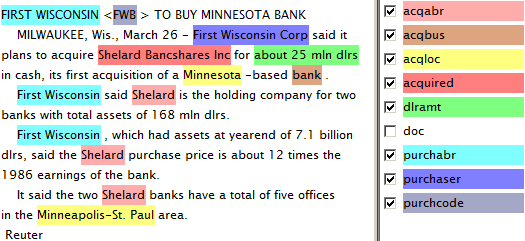
\includegraphics[width=0.75\hsize]{acquisitions_annotated}}
\caption{Annotations of Corporate Acquisition Events}
\label{fig:acquisitions_annotated}
\end{figure}


\begin{figure}[p]
\centering
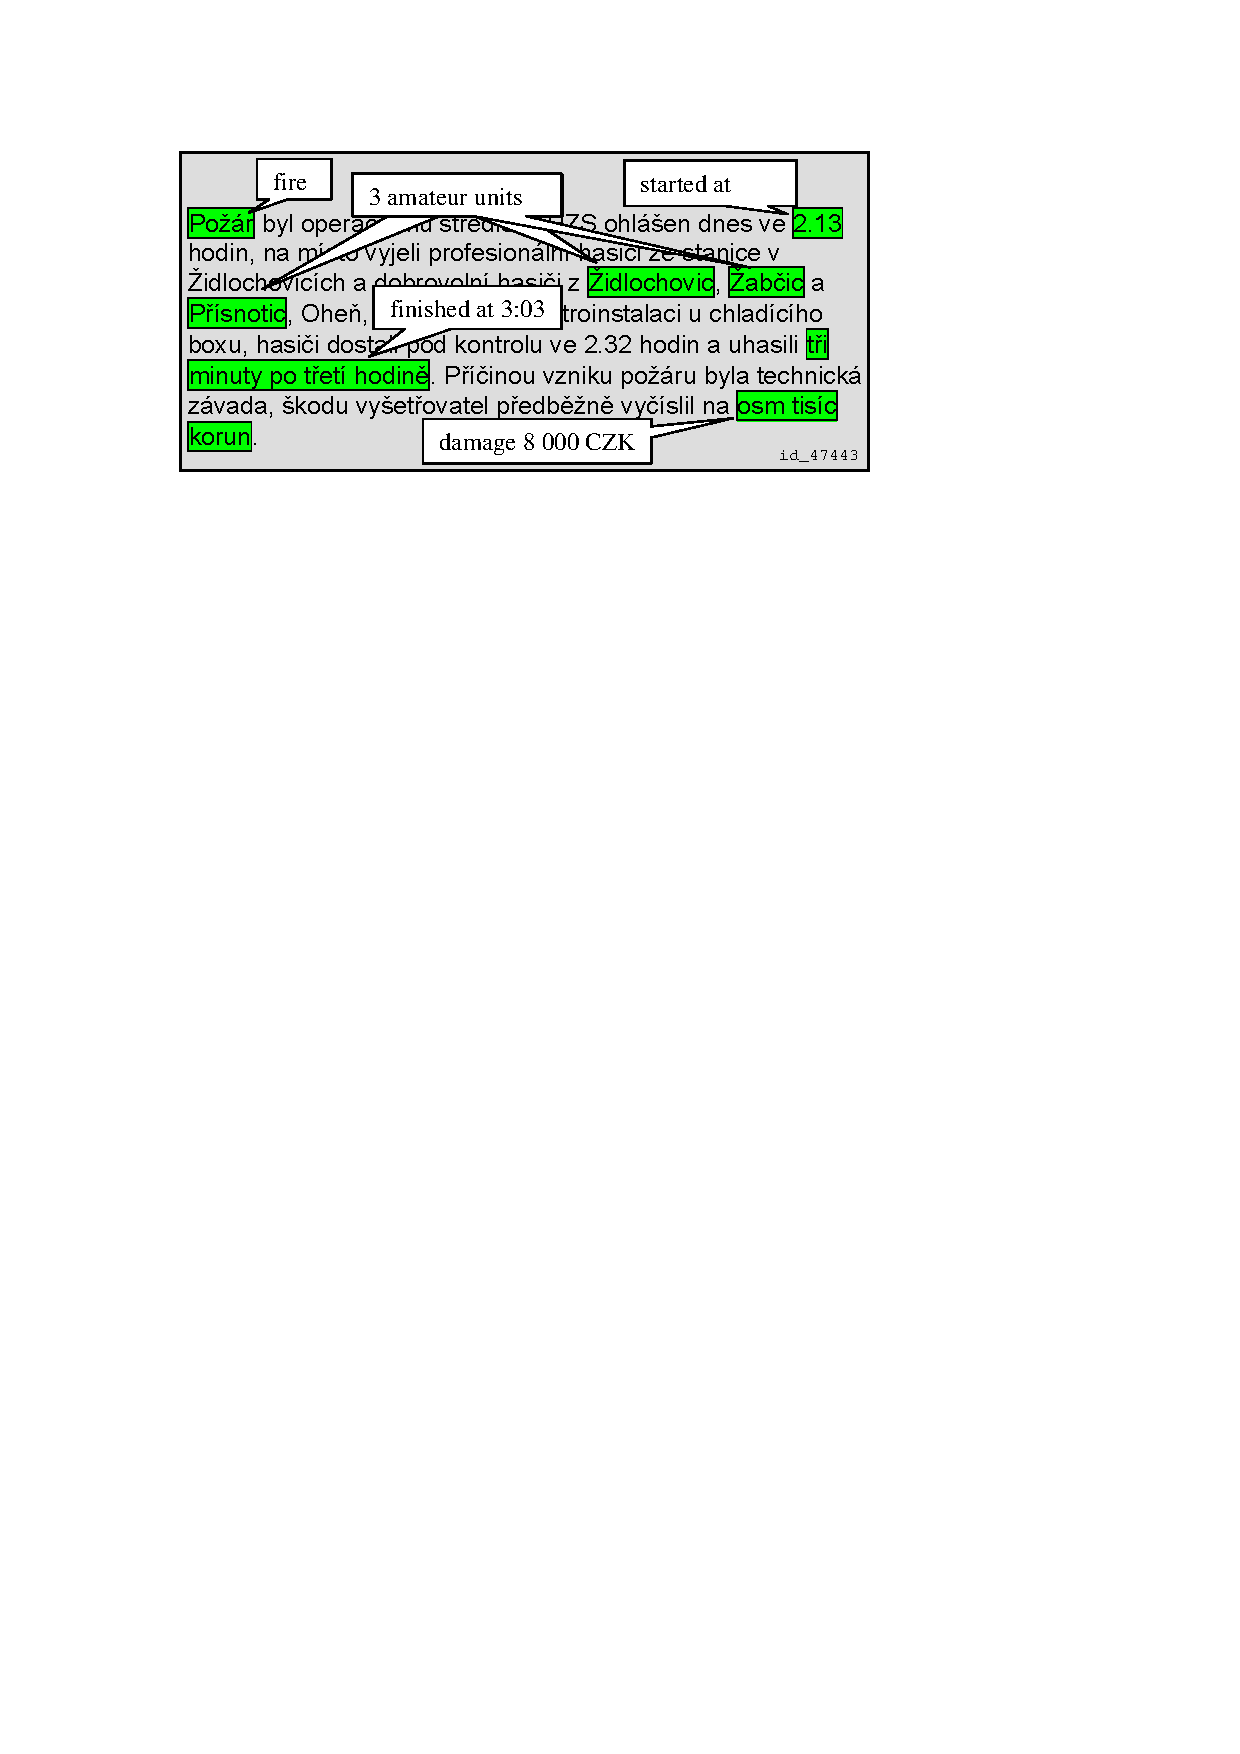
\includegraphics[width=0.65\hsize]{fireman_annotated}
\caption{Annotations of Czech Fireman events}
\label{fig:fireman_annotated}
\end{figure}


\begin{figure}[p]
\centerline{\framebox{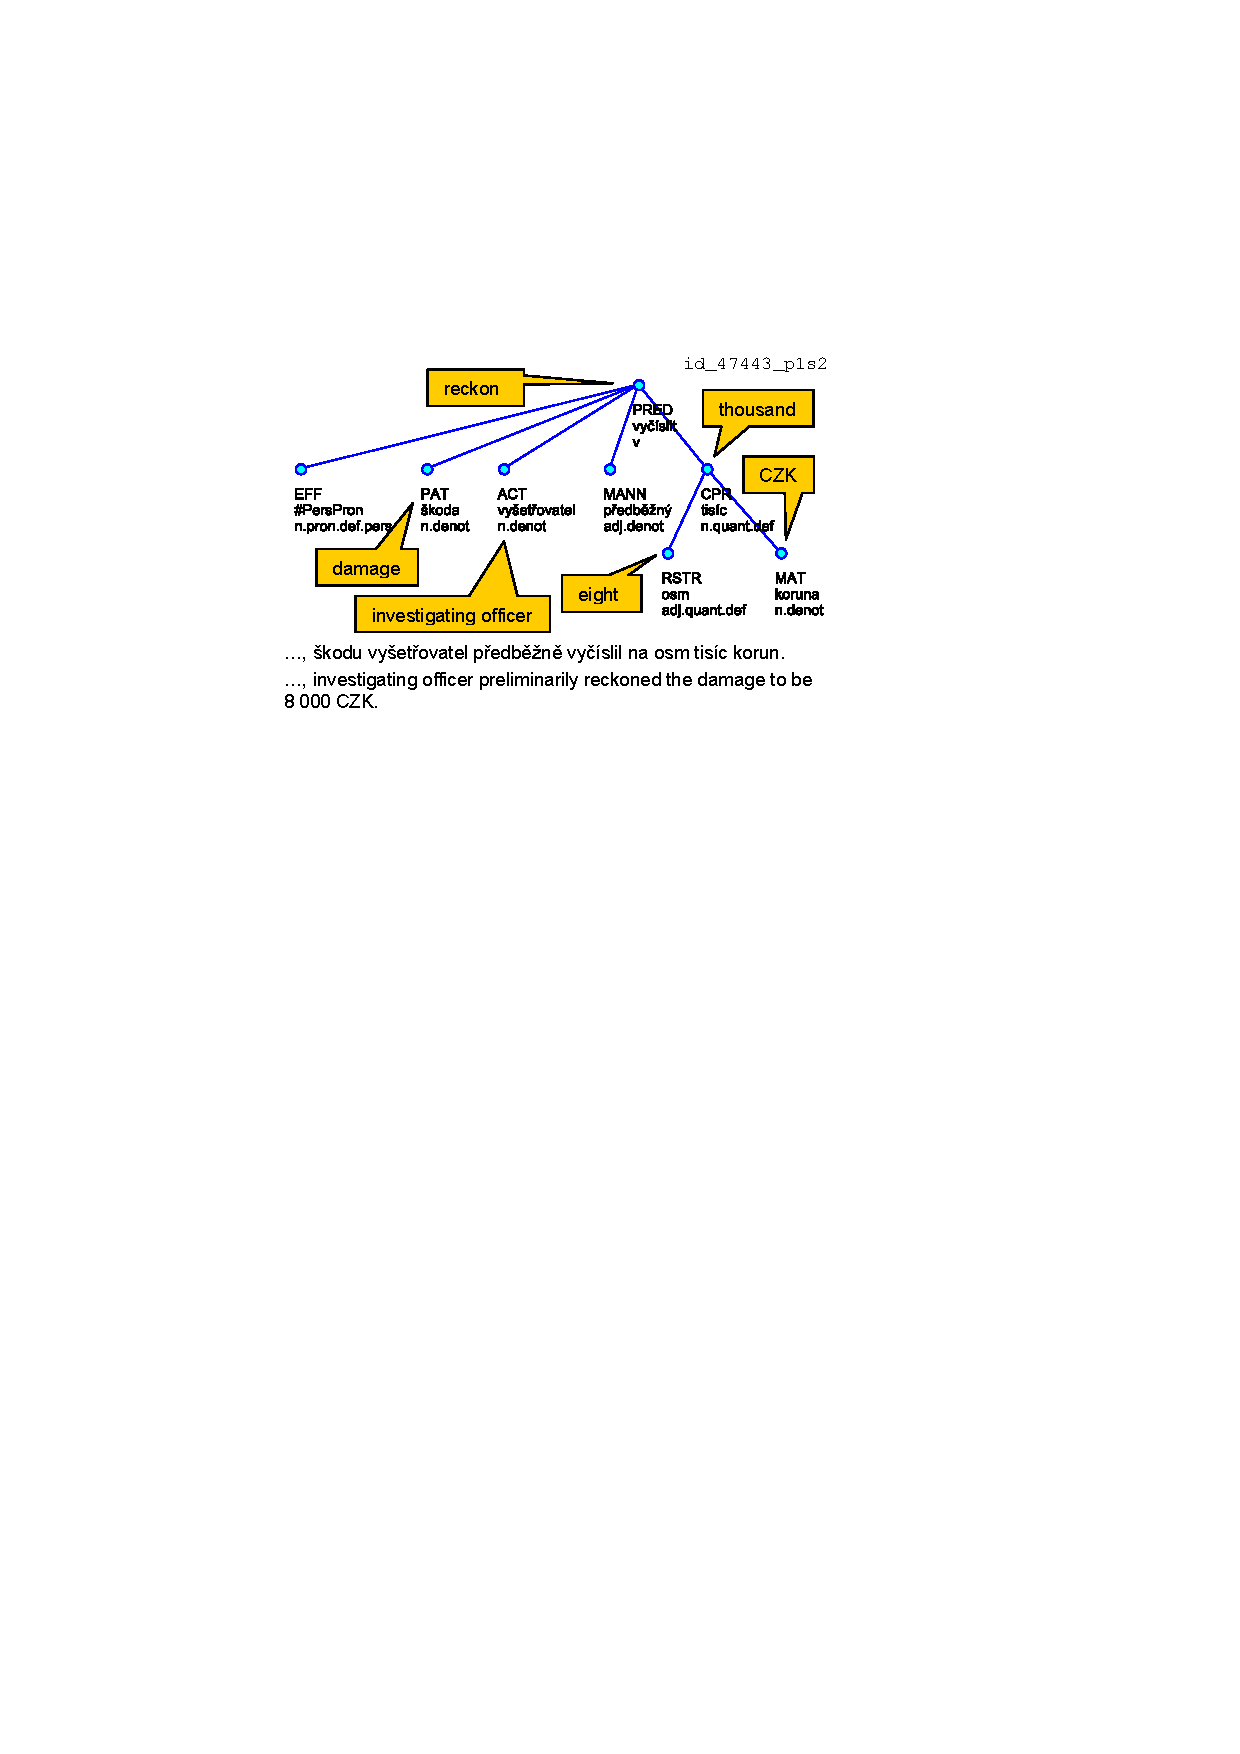
\includegraphics[width=0.7\hsize]{damage_tree}}}
\caption{Example of a linguistic tree of one analyzed sentence.}
\label{fig:intro_damage_tree} 
\end{figure}


%\subsection{Motivation of Our Approaches}

The main motivation for creating our extraction methods was an attempt to use deep linguistic analysis for this task. Especially for the Czech language with free word order this seemed reasonable. It is much more straightforward to design extraction rules on the basis of linguistic dependency trees than to struggle with the surface structure of text. In a dependency tree, the position of a word is determined by its syntactic (analytical trees) or even semantic role (tectogrammatical trees). So the extraction rules might not be dramatically affected by minor variations of the word order.

%\subsection{Usage}
Besides that information extraction and annotation is very interesting and challenging problem, it is also particularly useful. This period can be characterized by information overload and information extraction can provide partial answer to that. It provides fine grained indexing of documents, which supports precise search and document filtering. Navigation within individual documents can be faster and reading can be more effective. Other software programs can use the extracted information and perform additional computations resulting in summaries and answers integrated from different sources.  The effort in this direction will hopefully culminate in the realization of the idea of the Semantic Web, when all the information will be available in a machine workable form and the whole (semantic) web could be used as a huge knowledge base.



\section{Contribution} \label{sec:phd_contributions}

Let us briefly summarize the main contributions of the present work.

\subsection{New Ideas, Models and Methods}

Novel and original approaches or adaptations of existing ones are presented in this work.

\subsubsection{Manual Design of Extraction Rules}
The extraction method based on manually designed extraction rules is unique in the high expressiveness of extraction rules and the existence GUI (Graphical User Interface) for graphical design of these rules, both of these benefits are brought by the existence of the linguistic tool Netgraph \citep{biblio:MiNetgraphA2006}, which was exploited as the core of the extraction method.

\subsubsection{Machine Learning of Extraction Rules}
Very similar approaches to our extraction method based on ILP were already reported in literature \citep{DBLP:conf/ilp/RamakrishnanJBS07, aitken02:_learn_infor_extrac_rules}, but they were developed partly in parallel with our solution and they do not provide a publicly available and usable implementation. The method also represents the first attempt to use PDT (Prague Dependency Treebank) resources (e.g. tectogrammatical trees \citep{biblio:MiBeAnnotationtectogrammatical2006}) in the area of information extraction. Evaluation of the method on the language pair of Czech and English demonstrates its language independence.

\subsubsection{Shareable Extraction Ontologies}
The topic of shareable extraction ontologies introduces completely new paradigm to the design and usage of extraction ontologies \citep{DBLP:conf/er/EmbleyTL02}. The usage of a semantic web reasoner as the interpreter of an extraction ontology has never been demonstrated before.


\subsubsection{Fuzzy ILP Classification}
Last but not least, the attempt to use information extracted from a document for document classification is also reported for the first time, although our attention is more focused on the implementation and evaluation of the Fuzzy ILP Classifier based on the sound theory of fuzzy logic \citep{biblio:Hajek} and fuzzy ILP \citep{biblio:FILP}.



\subsection{New Software}

As a part of our work, new publicly available implementation of the described methods was created. 

A simple and extensible API (Application Programming Interface) interface of the extraction method based on manually designed extraction rules is provided such that users can design extraction rules in the Netgraph GUI and evaluate them on the whole corpus using this interface. 

The extraction method based on ILP is fully integrated in GATE (a widely used framework for text engineering \citep{biblio:GATE_ACL2002}) and it can be used as any other machine learning algorithm inside the framework. Moreover integration of TectoMT linguistic tools \citep{biblio:ZaPtTectoMTHighly2008} as well as the Netgraph tree viewer to the GATE framework was realized. Our implementation also provides utility functions for  comparative information extraction experiments using the cross-validation technique and investigation of statistical significance. 

The implementation of the case study with shareable extraction ontologies is not that general as the rest of the software part of our work but it can be easily followed and reproduced in similar experiments.

The implementation of the Fuzzy ILP Classifier is fully compatible with Weka (a widely used framework for machine learning experiments \citep{biblio:Weka}) and it can be used as any other Weka classifier, it also provides the possibility of custom integration of the classifier to an existing installation of the Weka system on the user's computer.

\subsection{New Data}

Several new datasets were established as a part of our work. We only list them here (see bellow), descriptions are available in the thesis.

\begin{itemize}
	\item Czech Fireman Reports without Annotations 
	\item Czech Fireman Reports Manually Annotated 
	\item RDF Dataset Based on Czech Fireman Reports 
	\item RDF Dataset Based on Corporate Acquisition Events 
	\item Classification Dataset Based on Czech Fireman Reports 
\end{itemize}

\subsection{Exploitation of Existing Resources}

Work of other researchers was exploited, extended and/or evaluated in the present work. For example our extraction methods represent the first application of PDT resources (e.g. Netgraph, tectogrammatical trees, etc.) in the area of information extraction. Comprehensive experiments were performed e.g. with the PAUM extraction algorithm \citep{Li:Paum}, with various semantic web reasoners (Jena\footnote{\url{http://jena.sourceforge.net}}
,HermiT\footnote{\url{http://hermit-reasoner.com}}
,Pellet\footnote{\url{http://clarkparsia.com/pellet}}
and FaCT++\footnote{\url{http://code.google.com/p/factplusplus}}), Weka classifiers (Multilayer Perceptron \citep{biblio:bishop-1995},
Support Vector Machine classifier SMO \citep{biblio:SMO},
J48 decision tree \citep{biblio:J48},
JRip rules \citep{weka:JRip} and
Additive logistic regression LogitBoost \citep{biblio:LogitBoost}), etc.

\subsection{Evaluation Experiments}

All approaches presented in the thesis were evaluated such that readers can obtain clear picture abut the performance and usability of these approaches. Most evaluation experiments are detailed and comprehensive, investigating also the statistical significance of the results.

\subsection{Publications and New Publicly Available Resources}

Majority of topics presented in the thesis were already published (going through peer review process), presented and discussed with international audience. Moreover several citations can be found in the literature showing that the work is already contributing to the generally available knowledge. See the attached list of publications (page~\pageref{sec:my_publications}).

Also the software and data parts of our work are publically available on the web, see details on the project's home page\footurl{http://czsem.berlios.de/}.  


\section{Conclusion}

Instead of focusing on a single topic and developing it in depth, the thesis has rather broader scope, even though many interesting ideas that came to our minds could not be investigated at all. For example the possibility to perform customized sentence clustering based on the syntactic tree structure could, supported by a handy GUI, result in a powerful tool for manual design of information extraction rules. We also could not develop any web information extraction approach exploiting the HTML structure, which, in combination with topological information about the placement of the elements on the screen, or even OCR, could bring new and interesting solution. We are pleased to share our best experience using the thesis, which includes:

\begin{itemize}
	\item Rather practically oriented information extraction method based on deep language parsing and manually designed extraction rules.

	\item A challenge presented by the attempt to beat the performance of other information extraction system by our method based on Inductive Logic Programming.  Let us note that the method touched the state-of-the-art in some cases but its time requirements are rather farther from it.

	\item Agitation brought by the presentation of something completely new, visionary and ``unconventional'', the idea of shareable extraction ontologies.

	\item Again a challenge connected with the evaluation of the Fuzzy ILP Classifier with the same result of touching the state-of-the-art (in some cases) and high time requirements; and also the experience with the implementation of formal mathematics with the result in a piece of working software (see the implementation details inside of the thesis.)
\end{itemize}


%%%%%%%%%%%%%%%%%%%%%%%%%%%%%%%%%%%%%%%%%%%%%%%%%%%%%%%%%%%%%%%%%%%%%%%
% Bibliography
%%%%%%%%%%%%%%%%%%%%%%%%%%%%%%%%%%%%%%%%%%%%%%%%%%%%%%%%%%%%%%%%%%%%%%%

%\myaddchaptertoc{Bibliography}
\bibliographystyle{../style/iisproc}
\bibliography{../dedek_phd}

%%%%%%%%%%%%%%%%%%%%%%%%%%%%%%%%%%%%%%%%%%%%%%%%%%%%%%%%%%%%%%%%%%%%%%%%%%%%%%%
%%%%%%%%%%%%%%%%%%%%%%%%%%%%%%%%%%%%%%%%%%%%%%%%%%%%%%%%%%%%%%%%%%%%%%%%%%%%%%%

\newpage

\section*{Publications} \label{sec:my_publications}

\subsubsection*{Refereed (English)}

\begin{itemize}


\item
Jan D{\v{e}}dek, Peter Vojt{\'{a}}{\v{s}}, and Marta Vomlelov{\'{a}}.
\newblock Fuzzy {ILP} classification of web reports after linguistic text
  mining.
\newblock {\em Information Processing \& Management}, 48\penalty0 (3):\penalty0
  438 -- 450, 2012.
\newblock Soft Approaches to IA on the Web.
\newblock Available from:
  \url{http://www.sciencedirect.com/science/article/pii/S0306457311000264}.


\item
Jan D{\v{e}}dek.
\newblock Towards semantic annotation supported by dependency linguistics and
  {ILP}.
\newblock In {\em Proceedings of the 9th International Semantic Web Conference
  (ISWC2010), Part II}, volume 6497 of {\em Lecture Notes in Computer Science},
  pages 297--304, Shanghai / China, 2010. Springer-Verlag Berlin Heidelberg.
\newblock ISBN 978-3-642-17748-4.
\newblock Available from:
  \url{http://iswc2010.semanticweb.org/accepted-papers/219}.

\item
Jan D{\v{e}}dek and Peter Vojt{\'{a}}{\v{s}}.
\newblock Semantic annotation semantically: Using a shareable extraction
  ontology and a reasoner.
\newblock In Pascal Lorenz and Eckhard Ammann, editors, {\em {SEMAPRO 2011},
  The Fifth International Conference on Advances in Semantic Processing}, pages
  29--34. (c) {IARIA}, {XPS}, 2011.
\newblock ISBN 978-1-61208-175-5.
\newblock Available from:
  \url{http://www.thinkmind.org/index.php?view=article&articleid=semapro_2011_2_10_50013}.



\item
Jan D{\v{e}}dek and Peter Vojt{\'{a}}{\v{s}}.
\newblock Linguistic extraction for semantic annotation.
\newblock In Costin Badica, Giuseppe Mangioni, Vincenza Carchiolo, and Dumitru
  Burdescu, editors, {\em 2nd International Symposium on Intelligent
  Distributed Computing}, volume 162 of {\em Studies in Computational
  Intelligence}, pages 85--94, Catania, Italy, 2008. Springer-Verlag.
\newblock ISBN 978-3-540-85256-8.
\newblock Available from:
  \url{http://www.springerlink.com/content/w7213j007t416132}.


\item
Jan D{\v{e}}dek and Peter Vojt{\'{a}}{\v{s}}.
\newblock Computing aggregations from linguistic web resources: a case study in
  czech republic sector/traffic accidents.
\newblock In Cosmin Dini, editor, {\em Second International Conference on
  Advanced Engineering Computing and Applications in Sciences}, pages 7--12.
  {IEEE} Computer Society, 2008.
\newblock ISBN 978-0-7695-3369-8.
\newblock Available from: \url{http://dx.doi.org/10.1109/ADVCOMP.2008.17}.

\item
Jan D{\v{e}}dek and Peter Vojt{\'{a}}{\v{s}}.
\newblock Exploitation of linguistic tools in semantic extraction - a design.
\newblock In Mieczys{{\l}}aw K{{\l}}opotek, Adam Przepi{\'{o}}rkowski,
  S{{\l}}awomir Wierzcho{\'{n}}, and Krzysztof Trojanowski, editors, {\em
  Intelligent Information Systems {XVI}}, pages 239--247, Zakopane, Poland,
  2008. Academic Publishing House {EXIT}.
\newblock ISBN 978-83-60434-44-4.
\newblock Available from:
  \url{http://iis.ipipan.waw.pl/2008/proceedings/iis08-23.pdf}.


\item
Jan D{\v{e}}dek and Peter Vojt{\'{a}}{\v{s}}.
\newblock Fuzzy classification of web reports with linguistic text mining.
\newblock In Paolo Boldi, Giuseppe Vizzari, Gabriella Pasi, and Ricardo
  Baeza-Yates, editors, {\em Web Intelligence and Intelligent Agent Technology,
  IEEE/WIC/ACM International Conference on}, volume~3, pages 167--170, Los
  Alamitos, CA, USA, 2009. IEEE Computer Society.
\newblock ISBN 978-0-7695-3801-3.
\newblock Available from: \url{http://dx.doi.org/10.1109/WI-IAT.2009.254}.


\item
Jan D{\v{e}}dek, Alan Eckhardt, and Peter Vojt{\'{a}}{\v{s}}.
\newblock Experiments with czech linguistic data and {ILP}.
\newblock In Filip {\v{Z}}elezn{\'{y}} and Nada Lavra{\v{c}}, editors, {\em
  {ILP} 2008 - Inductive Logic Programming (Late Breaking Papers)}, pages
  20--25, Prague, Czech Republic, 2008. Action M.
\newblock ISBN 978-80-86742-26-7.
\newblock Available from:
  \url{http://ida.felk.cvut.cz/ilp2008/ILP08_Late_Breaking_Papers.pdf}.




\item
Jan D{\v{e}}dek, Alan Eckhardt, Leo Galambo{\v{s}}, and Peter
  Vojt{\'{a}}{\v{s}}.
\newblock Discussion on uncertainty ontology for annotation and reasoning (a
  position paper).
\newblock In P.~C.~G. da~Costa, editor, {\em {URSW} '08 Uncertainty Reasoning
  for the Semantic Web - Volume 4}, volume 423 of {\em {CEUR} Workshop
  Proceedings}, pages 128--129. The 7th International Semantic Web Conference,
  2008.
\newblock Available from:
  \url{http://c4i.gmu.edu/ursw/2008/papers/URSW2008_P2_DedekEtAl.pdf}.


\item
Jan D{\v{e}}dek.
\newblock Web information extraction systems for web semantization.
\newblock In Peter Vojt{\'{a}}{\v{s}}, editor, {\em {ITAT} 2009 Information
  Technologies - Applications and Theory}, pages 1--6, Se{\v{n}}a, Slovakia,
  2009. {PONT} Slovakia.
\newblock ISBN 978-80-970179-2-7.
\newblock Available from: \url{http://ceur-ws.org/Vol-584/paper1.pdf}.


\item
Jan D{\v{e}}dek and Peter Vojt{\'{a}}{\v{s}}.
\newblock Web information extraction for e-environment.
\newblock In Jiri Hrebicek, Jiri Hradec, Emil Pelikan, Ondrej Mirovsky, Werner
  Pillmann, Ivan Holoubek, and Thomas Bandholtz, editors, {\em Proceedings of
  the European conference of the Czech Presidency of the Council of the {EU
  TOWARDS eENVIRONMENT}}, pages 138--143, Brno, Czech Republic, 2009. Masaryk
  University.
\newblock ISBN 978-80-210-4824-9.
\newblock Available from: \url{http://www.e-envi2009.org/?proceedings}.







\end{itemize}

\subsubsection*{Refereed (Czech and Slovak)}

\begin{itemize}





\item
Jan D{\v{e}}dek and Peter Vojt{\'{a}}{\v{s}}.
\newblock Extrakce informac{\'{i}} z textov{\v{e}} orientovan{\'{y}}ch
  zdrojů webu.
\newblock In V{\'{a}}clav Sn{\'{a}}{\v{s}}el, editor, {\em Znalosti 2008},
  pages 331--334, 2008.
\newblock ISBN 978-80-227-2827-0.
\newblock Available from:
  \url{http://znalosti2008.fiit.stuba.sk/download/articles/znalosti2008-Dedek.pdf}.


\item
Jan D{\v{e}}dek, Peter Vojt{\'{a}}{\v{s}}, and Marta Vomlelov{\'{a}}.
\newblock Evaluace fuzzy {ILP} klasifik{\'{a}}toru na datech o dopravn{\'{i}}ch
  nehod{\'{a}}ch.
\newblock In Pavel Smr{\v{z}}, editor, {\em Znalosti 2010}, pages 187--190,
  Jind{\v{r}}ichův Hradec, 2010. V{\v{S}}E v Praze, Oeconomica.
\newblock ISBN 978-80-245-1636-3.



\item
Jan D{\v{e}}dek, Peter Vojt{\'{a}}{\v{s}}, and Juraj Vojt{\'{a}}{\v{s}}.
\newblock Obsahuje web indikace bl\'{i}\v{z}\'{i}c\'{i} se krize? {U}m\'{i}me
  je rozeznat?
\newblock In Ji\v{r}\'{i} Vo\v{r}\'{i}\v{s}ek, editor, {\em Syst\'{e}mov\'{a}
  integrace 2010}, pages 166--175, Praha, 2010. V{\v{S}}E v Praze, Oeconomica.
\newblock ISBN 978-80-245-1660-8.


\end{itemize}




















\newpage
%
%\section*{Citations}
%
%
%\begin{itemize}
%\item
%Alan Eckhardt, T.~Horv{\'{a}}th, and Peter Vojt{\'{a}}{\v{s}}.
%\newblock {PHASES}: A user profile learning approach for web search.
%\newblock In Tsau Lin, Laura Haas, R.~Motwani, A.~Broder, and H.~Ho, editors,
%  \emph{2007 {IEEE}/{WIC}/{ACM} International Conference on Web Intelligence -
%  {WI} 2007}, pages 780--783. {IEEE}, 2007{}.
%\newblock ISBN 0-7695-3026-5/07.
%\begin{itemize}
%
%\item
%\bibitem[Dokulil et~al.(2008)Dokulil, Yaghob, and Katreniakov\'{a}]{b:citace2}
%Jir\'{\i} Dokulil, Jakub Yaghob, and Jana Katreniakov\'{a}.
%\newblock Everything you ever wanted to learn from the semantic web but were
%  unable to ask.
%\newblock In \emph{ADVCOMP '08: Proceedings of the 2008 The Second
%  International Conference on Advanced Engineering Computing and Applications
%  in Sciences}, pages 21--26, Washington, DC, USA, 2008. IEEE Computer Society.
%\newblock ISBN 978-0-7695-3369-8.
%\newblock \doi{http://dx.doi.org/10.1109/ADVCOMP.2008.12}.
%
%\end{itemize}
%
%\item
%\bibitem[Vojt{\'{a}}{\v{s}} and Eckhardt(2009)]{bmy:VoEcUsingtuneable2009}
%Peter Vojt{\'{a}}{\v{s}} and Alan Eckhardt.
%\newblock Using tuneable fuzzy similarity in non-metric search.
%\newblock In Tom{\'{a}}{\v{s}} Skopal and Pavel Zezula, editors, \emph{{SISAP}
%  2009: Second international workshop on similarity search and applications},
%  pages 163--164, Prague, Czech Republic, 2009. {IEEE}.
%\newblock ISBN 978-0-7695-3765-8.
%
%\begin{itemize}
%\item
%\bibitem[Skopal and Bustos(2010)]{b:citace1}
%Tomas Skopal and Benjamin Bustos.
%\newblock On nonmetric similarity search problems in complex domains.
%\newblock To appear in \emph{ACM Computing Surveys}, 2010.
%
%\end{itemize}
%
%
%
%\item
%Alan Eckhardt, T.~Horv{\'{a}}th, and Peter Vojt{\'{a}}{\v{s}}.
%\newblock Learning different user profile annotated rules for fuzzy preference
%  top-k querying.
%\newblock In H.~Prade and V.~Subrahmanian, editors, \emph{International
%  Conference on Scalable Uncertainty Management}, volume 4772 of \emph{Lecture
%  Notes In Computer Science}, pages 116--130, Washington {DC}, {USA},
%  2007{}. Springer Berlin / Heidelberg.
%\newblock ISBN 978-3-540-75407-7.
%
%\begin{itemize}
%\item
%\bibitem[Barla and Bieliková(2009)]{b:citace3}
%Michal Barla and Mária Bieliková.
%\newblock M.: Rule-based user characteristics acquisition from.
%\newblock In \emph{Logs With Semantics for Personalized Web-based Systems.
%  Computing and Informatics}, 2009.
%
%\end{itemize}
%
%
%
%\end{itemize}

%
%\newpage
%
%\section*{Ji\v{r}\'{i} Dokulil - Curriculum Vitae}
%
%\noindent
%Department of Software Engineering\\
%Faculty of Mathematics and Physics\\
%Charles University in Prague
%
%\vspace{8pt}
%\noindent
%\emph{Phone:} +420 221 914 271
%
%\vspace{8pt}
%\noindent
%\emph{Fax:} +420-221-914-323
%
%\vspace{8pt}
%\noindent
%\emph{E-mail:} \TheAuthorMail
%
%\vspace{8pt}
%\noindent
%\emph{Work address:} Malostransk\'{e} n\'{a}m. 25, 118 00, Praha 1, Czech Republic
%
%\vspace{8pt}
%\noindent
%\emph{Home address:} U Hradiska 7, 779 00, Olomouc, Czech Republic
%
%\vspace{8pt}
%\noindent
%\emph{Date and place of birth:} May 21, 1982, Olomouc, Czech Republic
%
%
%\subsubsection*{Education}
%
%\begin{itemize}
%\item \emph{2001--2006} Master's degree, software systems, Faculty of Mathematics and Physics, Charles University in Prague\\
%\emph{Master's thesis:} RDF querying (awarded 3rd place at SVO\v{C} 2006)
%\end{itemize}
%
%\subsubsection*{Research experience}
%
%\begin{itemize}
%\item \emph{2009 onwards:} Parallel data processing\\
%Bobox framework
%\item \emph{2005 onwards:} RDF querying\\
%SPARQL evaluation and indexing\\
%Trisolda query interface: A relational query inteface for RDF\\
%TriQ algebra: An algebra for RDF querying akin to relational algebra\\
%TriQuery language: A extension of XQuery for RDF querying
%\item \emph{2007--2009:} RDF visualization\\
%Trisolda RDF visualizer: A visualizer for large RDF data
%\item \emph{2004--2006:} Data integration\\
%DataPile: A universal storage architecture
%\end{itemize}
%
%\subsubsection*{Teaching experience}
%
%\begin{itemize}
%\item Compiler principles
%\item Parallel programming
%\item Object-oriented programming; C/C++
%\item Supervisor: 8 bachelor and master theses
%
%\end{itemize}
%
%\subsubsection*{Program committee membership}
%
%\begin{itemize}
%\item SEMAPRO 2009, 2010 conferences
%\item ITAT 2009, 2010 conferences
%\item ADVCOMP 2008 conference
%\end{itemize}
%
%\subsubsection*{Organizing committee membership}
%
%\begin{itemize}
%\item SOFSEM 2009 conference
%\end{itemize}

%%%%%%%%%%%%%%%%%%%%%%%%%%%%%%%%%%%%%%%%%%%%%%%%%%%%%%%%%%%%%%%%%%%%%%%%%%%%%%%

\end{document}

%%%%%%%%%%%%%%%%%%%%%%%%%%%%%%%%%%%%%%%%%%%%%%%%%%%%%%%%%%%%%%%%%%%%%%%%%%%%%%%
%%%%%%%%%%%%%%%%%%%%%%%%%%%%%%%%%%%%%%%%%%%%%%%%%%%%%%%%%%%%%%%%%%%%%%%%%%%%%%%


